\documentclass[border=15pt, multi, tikz]{standalone}
\usepackage{import}
\subimport{./layers/}{init}
\usetikzlibrary{positioning}
\usetikzlibrary{3d} %for including external image 

\def\ConvColor{rgb:yellow,5;red,2.5;white,5}
\def\ConvReluColor{rgb:yellow,5;red,5;white,5}
\def\PoolColor{rgb:red,1;black,0.3}
\def\DcnvColor{rgb:blue,5;green,2.5;white,5}
\def\SoftmaxColor{rgb:magenta,5;black,7}
\def\SumColor{rgb:blue,5;green,15}

\begin{document}
\begin{tikzpicture}
\tikzstyle{connection}=[ultra thick,every node/.style={sloped,allow upside down},draw=\edgecolor,opacity=0.7]
%%%%%%%%%%%%%%%%%%%%%%%%%%%%%%%%%%%%%%%%%%%%%%%%%%%%%%%%%%%%%%%%%%%%%%%%%%%%%%%%%%%%%%%%
%% Draw Layer Blocks
%%%%%%%%%%%%%%%%%%%%%%%%%%%%%%%%%%%%%%%%%%%%%%%%%%%%%%%%%%%%%%%%%%%%%%%%%%%%%%%%%%%%%%%%
\node[canvas is zy plane at x=0] (temp) at (-3,0,0) {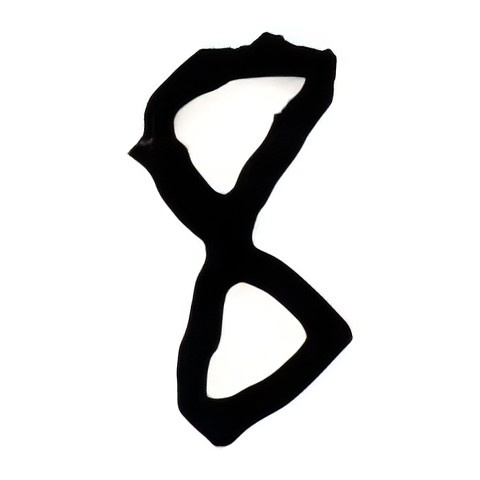
\includegraphics[width=8cm,height=8cm]{8.jpg} };
% conv1_1,conv1_2,%pool1
% Input Layer
% \pic[shift={(0,0,0)}] at (input-east) {RightBandedBox={
%     name=input,
%     caption=Input,
%     xlabel={{30, }},
%     zlabel=30,
%     fill=\ConvColor,
%     bandfill=\ReluColor,
%     height=30,
%     width=1,
%     depth=30
%     }
% };

% First convolution layer (first channel)
\pic[shift={(1,0,0)}] at (fircon-first-channe) {RightBandedBox={
    name=conv1a,
    caption=Conv1a,
    xlabel={{28, }},
    zlabel=28,
    fill=\ConvColor,
    bandfill=\ReluColor,
    height=28,
    width=1,
    depth=28
    }
};

% Second convolution layer (first channel)
\pic[shift={(1.5,0,0)}] at (conv1a-east) {RightBandedBox={
    name=conv2a,
    caption=Conv2a,
    xlabel={{26, }},
    zlabel=26,
    fill=\ConvColor,
    bandfill=\ReluColor,
    height=26,
    width=1,
    depth=26
    }
};

% Third convolution layer (first channel)
\pic[shift={(2,0,0)}] at (conv2a-east) {RightBandedBox={
    name=conv3a,
    caption=Conv3a,
    xlabel={{24, }},
    zlabel=24,
    fill=\ConvColor,
    bandfill=\ReluColor,
    height=24,
    width=1,
    depth=24
    }
};

% First convolution layer (second channel)
\pic[shift={(0,2,0)}] at (input-north) {RightBandedBox={
    name=conv1b,
    caption=Conv1b,
    xlabel={{28, }},
    zlabel=28,
    fill=\ConvColor,
    bandfill=\ReluColor,
    height=28,
    width=1,
    depth=28
    }
};

% Second convolution layer (second channel)
\pic[shift={(1.5,0,0)}] at (conv1b-east) {RightBandedBox={
    name=conv2b,
    caption=Conv2b,
    xlabel={{26, }},
    zlabel=26,
    fill=\ConvColor,
    bandfill=\ReluColor,
    height=26,
    width=1,
    depth=26
    }
};

% Third convolution layer (second channel)
\pic[shift={(2,0,0)}] at (conv2b-east) {RightBandedBox={
    name=conv3b,
    caption=Conv3b,
    xlabel={{24, }},
    zlabel=24,
    fill=\ConvColor,
    bandfill=\ReluColor,
    height=24,
    width=1,
    depth=24
    }
};

% Flatten layer
\pic[shift={(2.5,0,-1)}] at (conv3a-east) {RightBandedBox={
    name=flatten,
    caption=Flatten,
    xlabel={{1152, }},
    fill=\ConvColor,
    bandfill=\ReluColor,
    height=1,
    width=1,
    depth=115.2
    }
};

% First fully connected layer
\pic[shift={(3.5,0,0)}] at (flatten-east) {RightBandedBox={
    name=fc1,
    caption=FC1,
    xlabel={{180, }},
    fill=\FcColor,
    bandfill=\ReluColor,
    height=1,
    width=1,
    depth=18
    }
};

% First ReLU layer
\pic[shift={(0.5,0,0)}] at (fc1-east) {RightBandedBox={
    name=relu1,
    caption=ReLU1,
    xlabel={{180, }},
    fill=\ReluColor,
    height=1,
    width=1,
    depth=18
    }
};

% Second fully connected layer
\pic[shift={(1.5,0,0)}] at (relu1-east) {RightBandedBox={
    name=fc2,
    caption=FC2,
    xlabel={{45, }},
    fill=\FcColor,
    bandfill=\ReluColor,
    height=1,
    width=1,
    depth=4.5
    }
};

% Second ReLU layer
\pic[shift={(0.5,0,0)}] at (fc2-east) {RightBandedBox={
    name=relu2,
    caption=ReLU2,
    xlabel={{45, }},
    fill=\ReluColor,
    height=1,
    width=1,
    depth=4.5
    }
};

% Third fully connected layer
\pic[shift={(1.5,0,0)}] at (relu2-east) {RightBandedBox={
    name=fc3,
    caption=FC3,
    xlabel={{10, }},
    fill=\FcColor,
    bandfill=\ReluColor,
    height=1,
    width=1,
    depth=5%10
    }
};

% Output
\pic[shift={(2,0,0)}] at (fc3-east) {RightBandedBox={
    name=output,
    caption=Output,
    xlabel={{10, }},
    fill=\SoftmaxColor,
    bandfill=\SoftmaxColor,
    height=1,
    width=1,
    depth=5%10
    }
};

%%%%%%%%%%%%%%%%%%%%%%%%%%%%%%%%%%%%%%%%%%%%%%%%%%%%%%%%%%%%%%%%%%%%%%%%%%%%%%%%%%%%%%%%
%% Draw connections
%%%%%%%%%%%%%%%%%%%%%%%%%%%%%%%%%%%%%%%%%%%%%%%%%%%%%%%%%%%%%%%%%%%%%%%%%%%%%%%%%%%%%%%%
\draw [connection]  (input-east)    -- node {\midarrow} (conv1a-west);
%\draw [connection]  (input-east)    -- node {\midarrow} (fircon-first-channe);
\draw [connection]  (conv1a-east)   -- node {\midarrow} (conv2a-west);
\draw [connection]  (conv2a-east)   -- node {\midarrow} (conv3a-west);
\draw [connection]  (input-north)   -- node {\midarrow} (conv1b-west);
\draw [connection]  (conv1b-east)   -- node {\midarrow} (conv2b-west);
\draw [connection]  (conv2b-east)   -- node {\midarrow} (conv3b-west);
\draw [connection]  (conv3a-east)   -- node {\midarrow} (flatten-west);
\draw [connection]  (conv3b-west)   -- node {\midarrow} (flatten-west);
\draw [connection]  (flatten-east)  -- node {\midarrow} (fc1-west);
\draw [connection]  (fc1-east)      -- node {\midarrow} (relu1-west);
\draw [connection]  (relu1-east)    -- node {\midarrow} (fc2-west);
\draw [connection]  (fc2-east)      -- node {\midarrow} (relu2-west);
\draw [connection]  (relu2-east)    -- node {\midarrow} (fc3-west);
\draw [connection]  (fc3-east)      -- node {\midarrow} (output-west);
%%%%%%%%%%%%%%%%%%%%%%%%%%%%%%%%%%%%%%%%%%%%%%%%%%%%%%%%%%%%%%%%%%%%%%%%%%%%%%%%%%%%%%%%

\end{tikzpicture}
\end{document}\grid
